\documentclass{article}
\usepackage{hyperref}
\usepackage{graphicx}
\usepackage{geometry}
\usepackage{amsmath}
\newcommand\norm[1]{\left\lVert#1\right\rVert}
\usepackage{tikz}
\usepackage{float}
\tikzstyle{process} = [rectangle, minimum width=3cm, minimum height=1cm, text centered, draw=black, fill=orange!30]
\usetikzlibrary{shapes.geometric, arrows}
\tikzstyle{arrow} = [thick,->,>=stealth]
 \geometry{
 a4paper,
 total={170mm,257mm},
 left=30mm,
right=30mm,
 top=30mm,
bottom=15mm,
 }
\begin{document}
\title{Rain Removal Collections}
\author{Zhi Li}
\maketitle
\section{Single Image Based Methods}
\subsection{SPANet}
\href{https://arxiv.org/pdf/1904.01538.pdf}{Spatial Attentive Single-Image Deraining with a High Quality Real Rain Dataset}
\subsubsection{Key Points}
\begin{itemize}
\item Created Real Images 
\item Network (Attentive Network with four-directional feature map)
\end{itemize}
\subsubsection{Create real images}
since previous works are highly dependent on synthetic dataset to train the model, which is an ill-posed question. When their model is performed on real-world situation, they tend to be illy behaved, and of course not scaleable.\\
Author generates series of real world images to train. He extracts successive images at one rainfall event, and then dipicts histogram of every pixel, followed by manually inspection whether this pixel is occupied with rainfall or not because we understand that rain pixels are brighten.\\ \bigskip
%Flowchart goes here..
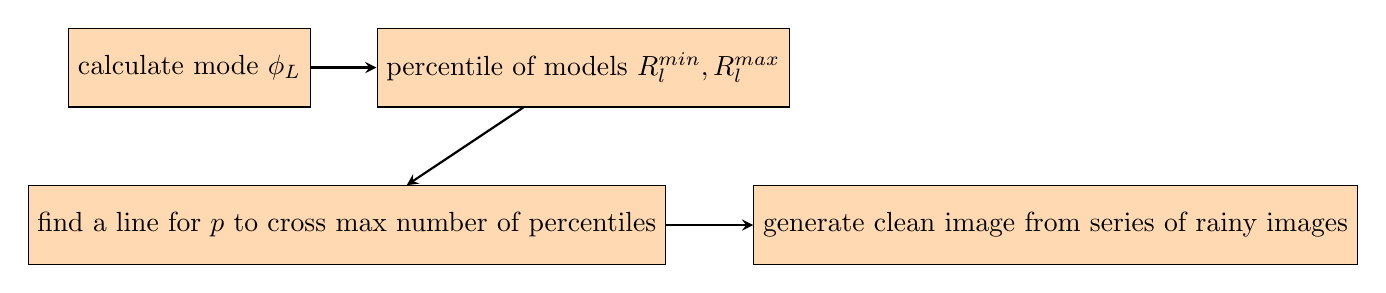
\begin{tikzpicture}[node distance=2cm]
\node (mode)[process]{calculate mode $\phi_L$ };
\node (percentile)[process, right of=mode, xshift=3cm]{percentile of models $R_l^{min},R_l^{max}$};
\node(line)[process, below of=mode, xshift=2cm]{find a line for $p$ to cross max number of percentiles};
\node(generate)[process, right of=line, xshift=7cm]{generate clean image from series of rainy images};
\draw [arrow] (mode) -- (percentile);
\draw [arrow] (percentile) -- (line);
\draw [arrow] (line) -- (generate);
\end{tikzpicture}

\subsubsection{Network}
``Recurrent neural networks with ReLU and identity matrix initialization (IRNN) for natural language processing have shown to be easy to train, good at long range dependencies as well as efficient. When applied to computer vision problems, their key advantage is that information can be efficiently propagated across the entire image to accumulate long range varing contextual information.''
\begin{figure}[H]
\centering
\includegraphics[width=\linewidth]{two-round-four-directional IRNN.PNG}
\caption{two-round four-directional IRNN schemetization}
\end{figure}
\begin{figure}[H]
\centering
\includegraphics[width=\linewidth]{SPANet}
\caption{Network description}
\end{figure}
\subsubsection{Loss Function}
\begin{equation}
L_{total}=L_1+L_{SSIM}+L_{Att}
\end{equation}
\begin{equation}
L_{Att}=\norm{A-M}_2
\end{equation}
where A is the attention map from the first SAM in the network andMis the binary map of the rain streaks, which is computed by thresholding the difference between the rain image and clean image. In this binary map, a 1 indicates that the pixel is covered by rain and 0 otherwise.

\subsection{JORDER}
\href{http://www.icst.pku.edu.cn/struct/Projects/joint_rain_removal.html}{Deep Joint Rain Detection and Removal from a Single Image}
\subsubsection{Key Points}
\begin{itemize}
\item seperate background learning and rain streak learning
\item network representing rainfall accumulation
\item recurrent rain detection and removal network
\end{itemize}
\subsubsection{Binary Rain Streak Map}
\begin{equation}
O=B+SR
\end{equation}
$SR$ is binary values, where 1 indicates rain regions and 0 indicates non-rain regions.''(1) it gives additional information for the network to learn about rain streak regions. (2) it allows a new rain removal pipeline to detect rain regions first, and the to operate differently on rain-streak and non-rain-streak regions, preserving background details.''
\subsubsection{Rain Accumulation and Heavy Rain}
\begin{equation}
O=\alpha(B+\sum_{t=1}^{s}{S_t}R)+(1-\alpha)*A
\end{equation}
t: overlapping streak number\\
s: number of shape and direction\\
A: global atmospheric light\\
$\alpha$: scene transmission\\
\subsubsection{Network}
\begin{figure}[H]
\centering
\includegraphics[width=\linewidth]{JORDEN}
\caption{JORDEN network schematizattion}
\end{figure}
For the training part, the author selected set of corresponding rain images, background images, rain regions maps and rain streak maps for training.
\subsubsection{Loss Function}
Multi-Task Objection Function
\begin{equation}
\operatorname*{argmin}_{B,S,R}\norm{O-B-SR}_2^2+P_b(B)+P_s(S)+P_r(R)
\end{equation}
\begin{equation}
L(\theta)=\frac{1}{n}(\norm{F_{rs}(o_i;\theta)-s_i}^2+\lambda_1\norm{F_{bg}(o_i;\theta)-g_i}^2-\lambda_2(log\hat{r}_{i,1}r_{i,1}+log(1-\hat{r}_{i,2})(1-r_{i,2})))
\end{equation}
with 
\begin{equation}
\hat{r}_{i,j}=\frac{exp{F_{rs}(o_i;\theta)}}{\sum_{k=1}^{2}exp{F_{rs,k}(o_i;\theta)}},j\in{\{1,2\}}
\end{equation}
Metrics Function: \href{https://en.wikipedia.org/wiki/Peak_signal-to-noise_ratio}{PSNR}, \href{https://en.wikipedia.org/wiki/Structural_similarity}{SSIM}
\subsection{Semi-supervised Transfer Learning for Single Image Rain Removal}
\href{https://arxiv.org/pdf/1807.11078.pdf}{Semi-supervised Transfer Learning for Single Image Rain Removal} attacks to provide two approaches, one supervised for paired no-rain and synthetic rain images, and the other unsupervised for real-world rainy images.
\subsubsection{Model Formulation}
Firstly, the author expresses the rain as Gaussian mixture model (GMM), because "GMM can be universal approximations to any continous functions if the parameters are learned appropriately."
\begin{equation*}
    R \sim  \sum_{k=1}^{K}\pi_{k}N(R \vert \mu_{k}, \sum_{k})
\end{equation*}

The negative log likelihood function imposed on these unsupervised samples can be written as


\begin{equation}
    L_{unsupervised}(R;\Pi,\Sigma) =-    \sum_{n=1}^{N}log        \sum_{k=1}^{K}\pi_{k}N(R_n \vert 0,\Sigma_{k})
\end{equation}
\subsubsection{Learning Diagram}
\begin{figure}[H]
    \centering
    \includegraphics[width=\linewidth]{semi-supervised_SIRR}
    \caption{schematic representation of the framework}
\end{figure}

\subsubsection{Loss Function}
For supervised paired loss, it is simple to adapt any norm loss like l1 loss or l2 loss. Hence, it can be formulated as follows.
\begin{equation*}
    L_{supervised}=\    \sum_{i=1}^{N} \vert\vert f_{w}(x_i)-y_i \vert\vert_{F}^{2}
\end{equation*}
However, for unlabelled learning, we should constrain the data distributions so that force generated domain not far from the real rain.


\begin{equation}
    D_{KL}(G_{syn}\vert\vert GMM_{real}) \simeq \min_{k}D_{KL}(G_{syn} \vert\vert GMM_{real}^k)
\end{equation}
Overall, the entire objective function to train the network is formulated as:


\begin{equation}
        L(w,\Pi,\Omega)=    \sum_{i=1}^{N_1}\vert\vert f_w(x_i)-y_i \vert\vert_F^2+ \alpha     \sum_{n=1}^{N_2}\vert\vert f_w(\hat{x}_n)\vert\vert_{TV}+\beta D_{KL}(G_x\vert\vert GMM_{\hat{x}})- \lambda     \sum_{n=1}^{N2}log     \sum_{k=1}^{K}\pi_kN(\hat{x}_n-f_w(\hat{x})_n\vert 0,\Omega_k)
\end{equation}



\subsection{D3RNet}
\href{http://www.icst.pku.edu.cn/struct/Pub%20Files/2019/ywh_tip19.pdf}{Dynamic Rounting Residue Recurrent Network for Video Rain Removal}
\subsubsection{Key Points}
\begin{itemize}
\item Dynamic Framework for video rain removal
\item Recurrent units to handle temporal fusion
\item Residual unit to compensate for negative rain features
\end{itemize}
\subsection{Model context}
\subsubsection{Occlusion-Aware Rain Model}
To address the occlusion effect caused by rain streaks, the author proposed a hybrid rain model which is adaptive to mdoel rain occlusions. All pixels in rain frames are classified into two groups: 1) the ones following the additive rain model the first equation; 2) the others whose pixel values are just equal to the rain reliance.
\begin{equation}
O_t=(1-\alpha)(B_t+S_t)+\alpha_tA_t
\end{equation}
\begin{equation}
\alpha_t(i,j)=
	\begin{cases}
		1 & \text{if $(i,j)\in \Omega_S$}\\
		0 & \text{if $(i,j)\not\in \Omega_S$}
	\end{cases}
\end{equation}
\subsubsection{Rain Removal Context}
''In our work, the difference of adjacent frames are used as a standard to classify motion regions. For groundtruth background frames, if the square of the difference of two adjacent frames is greater than 0.01, the region is denoted as motion regions.''

\subsection{Network}
\subsubsection{Spatial-Temporal Residue Recurrent Network}
\begin{figure}[H]
\centering
\includegraphics[width=\linewidth]{D3RNET.PNG}
\caption{Network architecture evoved from venilla convolutional neural network to our proposed spatial-temporal residue recurrent network}
\end{figure}

\begin{figure}[H]
\centering
\includegraphics[width=\linewidth]{D3RNET2.PNG}
\caption{D3RNet framework}
\end{figure}

\subsection{ReMAEN}
Single Image Deraining Using a Recurrent Multi-scale Aggregation and Enhancement Network

\subsubsection{Key Points}
\begin{itemize}
\item Reccurent blocks with shared channel attention
\item Detect multi-scale rain details
\item Edge loss is applied to preserve the background texture
\end{itemize}

\subsubsection{Network}
\begin{figure}[H]
\centering
\includegraphics[width=\linewidth]{ReMAEN}
\caption{Schematic Network description}
\end{figure}

\begin{equation}
\begin{split}
R_t= f_{ReMAEN}(I_{t-1})\, \\
I_t=I_{t-1}-R_t\\
\end{split}
\end{equation}

\subsubsection{Loss Function}
\begin{itemize}
\item MSE Loss \bigskip \\
No need to describe MSE loss here but the reason author applies more than MSE loss is because that MSE tends to blur out the image, and thus some details will be lost.
\item Edge Loss\\ \smallskip
\begin{equation}
L_{edge}=\frac{1}{HWC} \sum_{x=1}^{H} \sum_{y=1}^{W} \sum_{z=1}^{C} \vert \vert f(I_T)^{x,y,z}-f(I_{gt})^{x,y,z} \vert \vert^2
\end{equation}
Where the author defines the $f$ function as a edge detection kernel, see as follows,
\begin{equation}
K=
\begin{pmatrix}
-1 & -1 & -1 \\
-1 &  8 & -1  \\
-1 & -1 & -1   \\
\end{pmatrix}
\end{equation}

\end{itemize}

\subsection{PReNet}
\href{https://csdwren.github.io/papers/PReNet_cvpr_camera.pdf}{Progressive Image Deraining Networks: A Better and Simpler Baseline}

\end{document}

